\section{Die EV3-Steuereinheit}
%	\begin{figure}[h]
%		\begin{floatrow}
%			\ffigbox{%
%				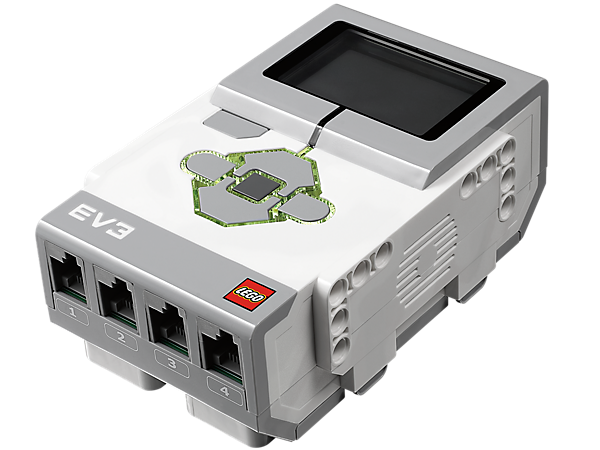
\includegraphics[width=9cm]{images/brick.png}%\rule{3cm}{3cm}%
%			}{%
%				\caption{EV3-Brick}%
%			}
%			\capbtabbox{%
%				\footnotesize
%				\begin{tabular}{|c|c|} \hline
%					Motorausg"ange & MotorPort.A \\
%					&MotorPort.B\\
%					&MotorPort.C\\
%					&MotorPort.D\\ \hline
%					Links & LEFT \\ \hline
%					Rechts & RIGHT \\ \hline
%					Oben & UP \\ \hline
%					Unten & DOWN \\ \hline
%					Mitte & ENTER \\ \hline
%					Oben-Links & ESCAPE \\ \hline
%					Sensoreing"ange & SensorPort.S1 \\
%					&SensorPort.S2\\
%					&SensorPort.S3\\
%					&SensorPort.S4\\ \hline
%				\end{tabular}
%			}{%
%				\caption{Tastenbenennung}%
%			}
%		\end{floatrow}
%	\end{figure}

	
	\begin{figure}[hptb]
		\begin{subfigure}{.65\textwidth}
			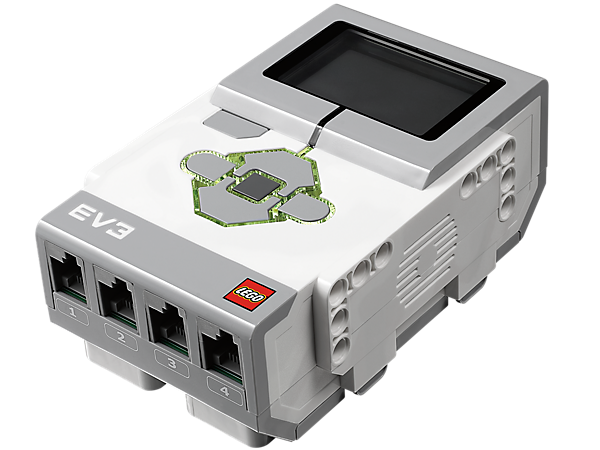
\includegraphics[width=\textwidth]{images/brick.png}
			\\
			\caption{EV3-Brick}
			\label{fig:g1}
		\end{subfigure}%
		\hfill
		\begin{subfigure}{.35\textwidth}
			%\centering
			\begin{tabular}{|c|c|} \hline
				Motorausg"ange & MotorPort.A \\
				&MotorPort.B\\
				&MotorPort.C\\
				&MotorPort.D\\ \hline
				Links & LEFT \\ \hline
				Rechts & RIGHT \\ \hline
				Oben & UP \\ \hline
				Unten & DOWN \\ \hline
				Mitte & ENTER \\ \hline
				Oben-Links & ESCAPE \\ \hline
				Sensoreing"ange & SensorPort.S1 \\
				&SensorPort.S2\\
				&SensorPort.S3\\
				&SensorPort.S4\\ \hline
			\end{tabular}
			\newline  \newline \newline \newline \newline
			\caption{Tastenbenennung}
			\label{fig:g2}
		\end{subfigure}
		%	\caption{Figure caption.}
	\end{figure}
	
	Durch Dr"ucken der mittleren und unteren Taste wird das laufende Programm beendet.
	

